\documentclass[twocolumn]{IEEEtran}
\usepackage{graphicx}
\usepackage[utf8x]{inputenc}
\usepackage{times}
\usepackage{amssymb,amsfonts}
\usepackage[tbtags]{amsmath}
\usepackage{cite}
\usepackage{pict2e}
\usepackage{float}
\usepackage{lscape}
\usepackage[all]{xy}
\usepackage{graphics,graphicx,color,colortbl}
\usepackage{times}
\usepackage{subfigure}
\usepackage{wrapfig}
%\usepackage{multicol}
\usepackage{cite}
\usepackage{url}
\usepackage[tbtags]{amsmath}
\usepackage{amsmath,amssymb,amsfonts,amsbsy}
\usepackage{listings}
\usepackage{bm}
\usepackage{algorithm}
\usepackage{algorithmic}
\usepackage[centerlast, small]{caption}
\usepackage[colorlinks=true, citecolor=blue, linkcolor=blue, urlcolor=blue, breaklinks=true]{hyperref}
\hyphenation{ele-men-tos he-rra-mi-en-ta cons-tru-yen trans-fe-ren-ci-a pro-pu-es-tas si-mu-lar vi-sua-li-za-cion}


\begin{document}
\title{Uso de la herramienta Electric VLSI}
\author{Nicolás David Arias Sosa \textbf{Código:} $261692$ \url{ndariass@unal.edu.co}\\
	David Ricardo Martínez Hernández \textbf{Código:} $261931$ \url{drmartinezhe@unal.edu.co}\\
	Oscar Alejandro Rojas Gallego \textbf{Código:} $xxxxxx$ \url{oarojasg@unal.edu.co}\\
	Universidad Nacional de Colombia}
\markboth{Uso de la herramienta Electric VLSI}{}
\maketitle

\begin{abstract}
En la práctica de laboratorio que se describe a continuación se realizaron los layouts de transistores MOSFET, de un inversor CMOS y de una compuerta de transmisión usando la herramienta \textit{Electric}. A partir de esto fue posible simular los modelos realizados en \textit{Spice}.
\end{abstract}
\begin{keywords}
 CMOS, Compuerta de transmisión, Compuerta Inversora, Tipo N y P, Transistor.
\end{keywords}

\section{Introducción}
\subsection{Reglas de diseño por capas sCMOS abstractas.}

En la tabla~\ref{t1scmos} y en la fig.~\ref{rulespng} se muestran las reglas a considerar en el diseño por capas sCMOS. Los valores presentados son dados en términos del parámetro $\lambda$, que para los diseños presentados es \textbf{300 nm}.

\newcolumntype{D}{ >{\arraybackslash} m{4cm} }
\begin{table}[H]
  \caption{Reglas de diseño por capas sCMOS abstractas.}
    \centering
      \begin{tabular}{|c|D|c|}\hline
       \bf Regla & \bf Descripción & \bf Valor ($\lambda$) \\ \hline
       3.1 & Ancho mínimo & 2 \\ \hline
       3.2 & Espacio mínimo & 2 \\ \hline
       3.2.a & Espacio mínimo sobre capa activa  & 2 \\ \hline 
       3.3 & Extensión mínima de compuerta sobre capa activa & 2 \\ \hline
       3.4 & Extensión mínima de capa activa sobre capa de polisilicio & 3 \\ \hline
       3.5 & Extensión mínima entre capas de polisilicio y activa & 1 \\ \hline
      \end{tabular}
  \label{t1scmos}
\end{table}

\begin{figure}[H]
  \centering
    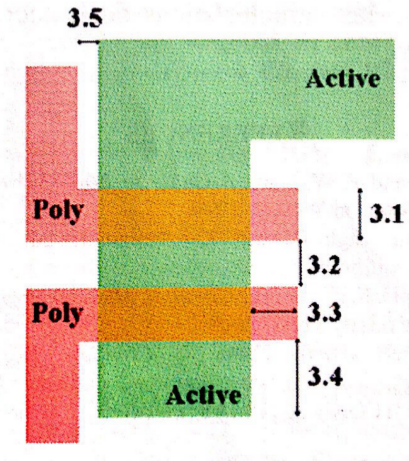
\includegraphics[scale=0.3]{pics/rules.png}
      \caption{Reglas de diseño en el diseño por capas sCMOS acorde a los valores de la tabla~\ref{t1scmos}.}
	\label{rulespng}
\end{figure}

\subsection{Relaciones de corriente en los transistores MOSFET.}
En las ecuaciones~\ref{idn}~y~\ref{idp} se muestran las relaciones de corriente para los transistores MOSFET N y P en modo de corte ($V_{gs} < |V_{th}|$), triodo ($|V_{ds}|<|V_{gs}|-|V_{th}|$) y saturación (caso contrario)

\footnotesize
\begin{equation}
I_{dn} = \left\{
  \begin{array}{lr}
  	0 & : \text{corte} \\
    k_n^{'}\dfrac{W}{L}\left((V_{gs}-|V_{th}|)V_{ds}-\dfrac{V_{ds}^{2}}{2} \right) & : \text{triodo} \\
    \dfrac{k_n^{'}}{2} \dfrac{W}{L}  \left( V_{gs} - |V_{th}| \right)^2  & : \text{saturación}
  \end{array}
\right.
\label{idn}
\end{equation}

\begin{equation}
I_{dp} = \left\{
  \begin{array}{lr}
  	0 &: \text{corte} \\
    k_n^{'}\dfrac{W}{L}\left((V_{sg}-|V_{th}|)V_{sd}-\dfrac{V_{sd}^{2}}{2} \right) &: \text{triodo} \\
    \dfrac{k_n^{'}}{2} \dfrac{W}{L}  \left( V_{sg} - |V_{th}| \right)^2  &: \text{saturación}
  \end{array}
\right.
\label{idp}
\end{equation}

\normalsize

\section{Transistor tipo P}
\noindent
Se realizó el diseño de un layout con un transistor P con $W$=3.6 $\mu$m y $L$=1.2 $\mu$m. El layout realizado se muestra en la fig.~\ref{layoutP}. A partir de esto se hizo la generación y simulación correspondiente del modelo en SPICE.

\begin{figure}[H]
  \centering
    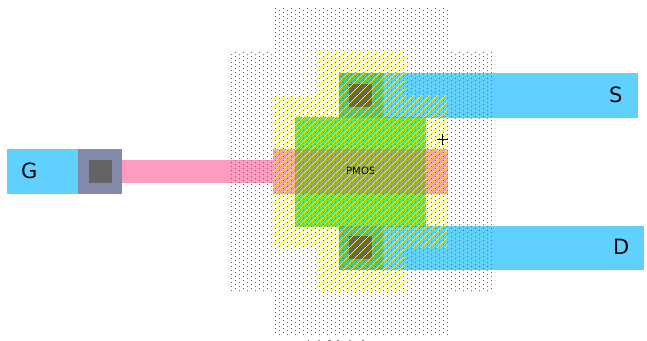
\includegraphics[scale=0.3]{pics/layoutP.png}
      \caption{Layout hecho en \textit{Electric} de un transistor P}
	\label{layoutP}
\end{figure}
\noindent
En la fig.~\ref{simP1} se muestra la gráfica $I_d$ vs. $V_{ds}$ para diferentes valores de $V_{gs}$ y en la fig.~\ref{simP2} se muestra la gráfica $I_d$ vs $V_{gs}$ para diferentes valores de $V_{ds}$. 

\begin{figure}[H]
  \centering
    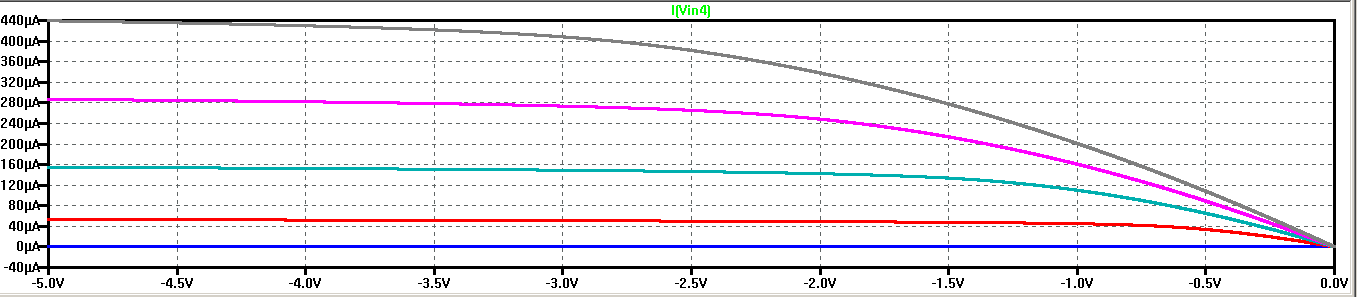
\includegraphics[scale=0.18]{pics/P_id_vds.png}
      \caption{Gráfico de $I_d$ vs. $V_{ds}$ para valores de $V_{gs}$ entre 0 V y 5 V.}
	\label{simP1}
\end{figure}

\begin{figure}[H]
  \centering
    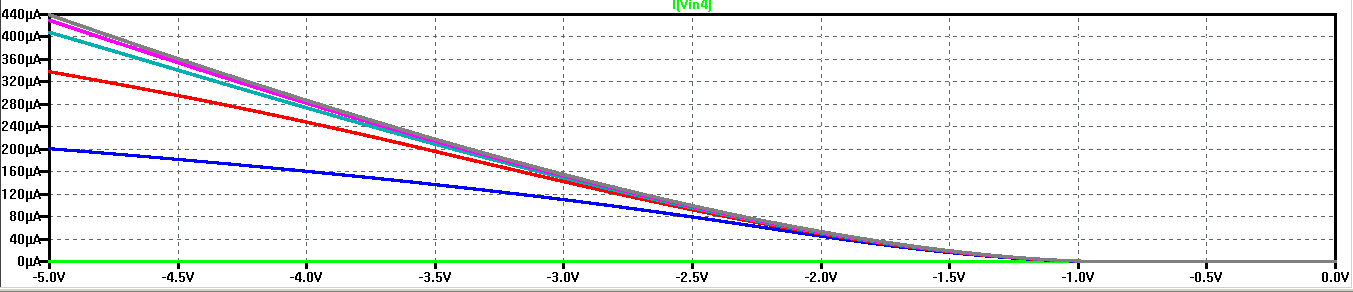
\includegraphics[scale=0.18]{pics/P_id_vgs.png}
      \caption{Gráfica de $I_d$ vs $V_{gs}$ para $V_{ds}$ entre 0 V y 5 V.}
	\label{simP2}
\end{figure}

\section{Transistor tipo N}
\noindent
Se realizó el diseño de un layout con un transistor N con $W$=3.6 $\mu$m y $L$=1.2 $\mu$m. El layout realizado se muestra en la fig.~\ref{layoutN}. A partir de esto se hizo la generación y simulación correspondiente del modelo en SPICE.

\begin{figure}[H]
  \centering
    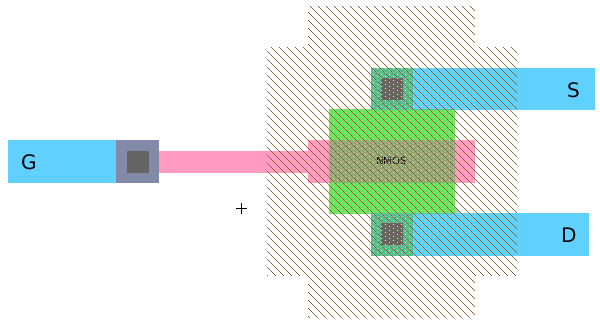
\includegraphics[scale=0.3]{pics/layoutN.png}
      \caption{Layout hecho en \textit{Electric} de un transistor N.}
	\label{layoutN}
\end{figure}
\noindent
En la fig.~\ref{simP3} se muestra la gráfica $I_d$ vs. $V_{ds}$ para diferentes valores de $V_{gs}$ y en la fig.~\ref{simP4} se muestra la gráfica $I_d$ vs $V_{gs}$ para diferentes valores de $V_{ds}$. 

\begin{figure}[H]
  \centering
    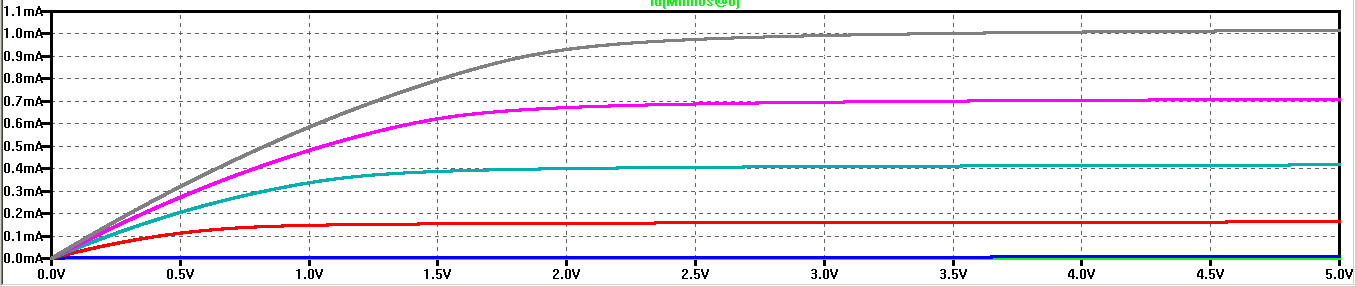
\includegraphics[scale=0.18]{pics/N_id_vds.png}
      \caption{Gráfico de $I_d$ vs. $V_{ds}$ para valores de $V_{gs}$ entre 0 V y 5 V.}
	\label{simP3}
\end{figure}

\begin{figure}[H]
  \centering
    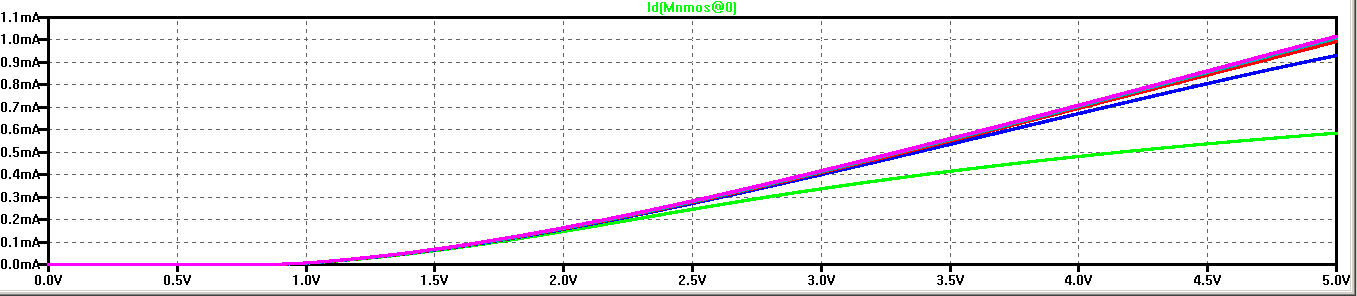
\includegraphics[scale=0.18]{pics/N_id_vgs.png}
      \caption{Gráfica de $I_d$ vs $V_{gs}$ para $V_{ds}$ entre 0 V y 5 V.}
	\label{simP4}
\end{figure}

\section{Inversor CMOS}
\noindent
Se realizó el diseño de un layout con un transistor P con $W=3\, \mu m$ y $L=0.6 \,\mu m$, para el transistor N con $W=1.5\, \mu m$ y $L=0.6 \,\mu m$. El layout realizado se muestra en la fig.~\ref{fig1}. A partir de esto se hizo la generación y simulación correspondiente del modelo en SPICE.
\begin{figure}[H]
  \centering
    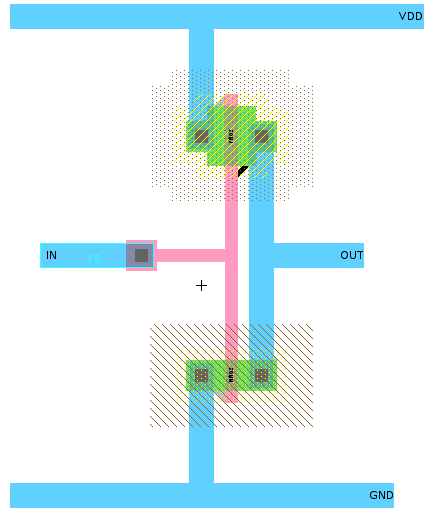
\includegraphics[scale=0.35]{pics/inversor.png}
      \caption{Layout hecho en \textit{Electric} de una compuerta inversora.}
	\label{fig1}
\end{figure}
\begin{figure}[H]
  \centering
    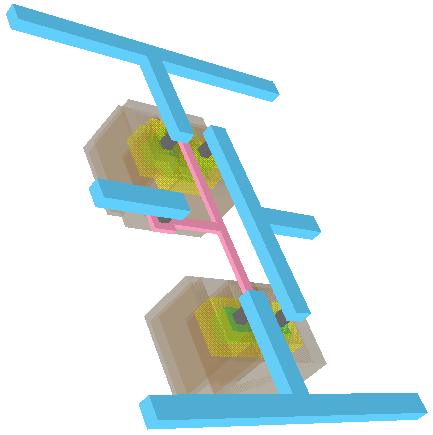
\includegraphics[scale=0.35]{pics/inversor3d.png}
      \caption{Layout hecho en \textit{Electric} de una compuerta inversora en su vista $3D$.}
	\label{fig2}
\end{figure}
\noindent
Para la primera siulacion se polarizó con un $V_{DD} = 5\, V$ dando como relustado
\begin{figure}[H]
  \centering
    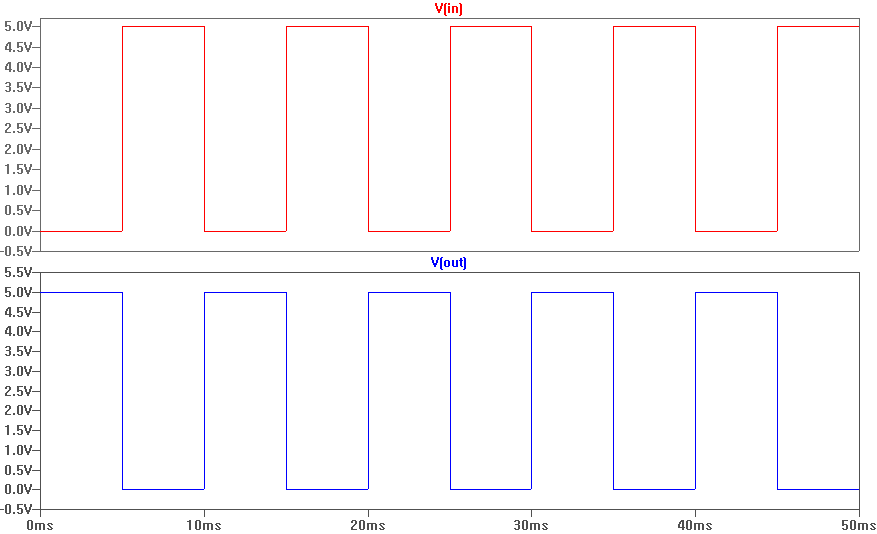
\includegraphics[scale=0.3]{pics/outinv.png}
      \caption{Comportamiento de la compuerta inversora del modelo SPICE.}
	\label{outinv}
\end{figure}
\begin{figure}[H]
  \centering
    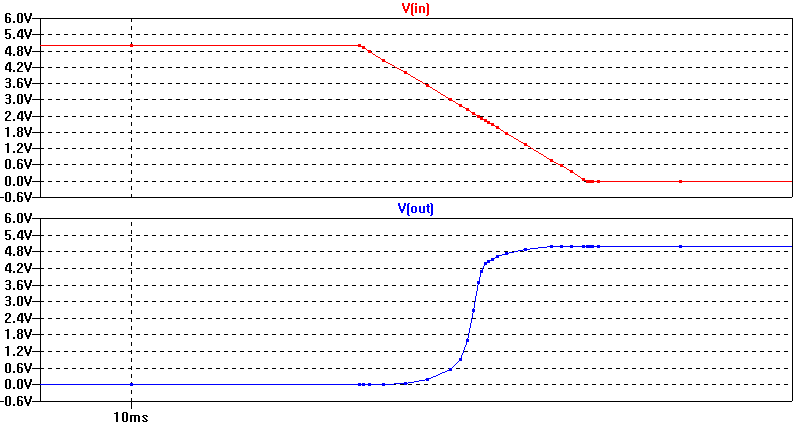
\includegraphics[scale=0.35]{pics/delay1.png}
      \caption{Retardo de las señales para $V_{DD}=5\, V$ para la compuerta inversora.}
	\label{delay1}
\end{figure}
\noindent
Para la primera simulación se polarizó con un $V_{DD} = 3\, V$ los resultados fueron los mismos resultados como los de la \ref{outinv} solo cambio el retardo del transistor (ver Fig.~\ref{dalay2})
\begin{figure}[H]
  \centering
    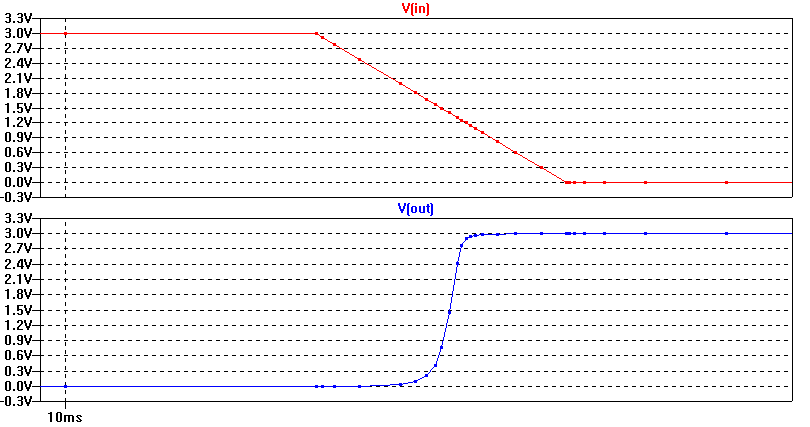
\includegraphics[scale=0.32]{pics/delay2.png}
      \caption{Retardo de las señales para $V_{DD}=3\, V$ para la compuerta inversora.}
	\label{delay2}
\end{figure}

\section{Compuerta de transmisión}
\noindent
Se realizó el diseño de un layout con un transistor P con $W=3\, \mu m$ y $L=0.6 \,\mu m$, para el transistor N con $W=1.5\, \mu m$ y $L=0.6 \,\mu m$. El layout realizado se muestra en la fig.~\ref{fig3}. A partir de esto se hizo la generación y simulación correspondiente del modelo en SPICE.
\begin{figure}[H]
  \centering
    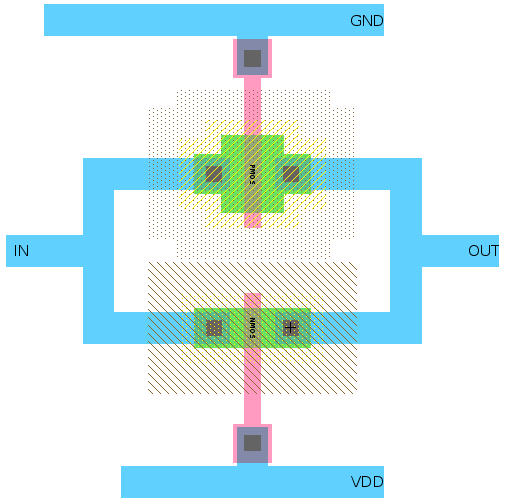
\includegraphics[scale=0.35]{pics/trans.png}
      \caption{Layout hecho en \textit{Electric} de una compuerta de transmisión.}
	\label{fig3}
\end{figure}
\begin{figure}[H]
  \centering
    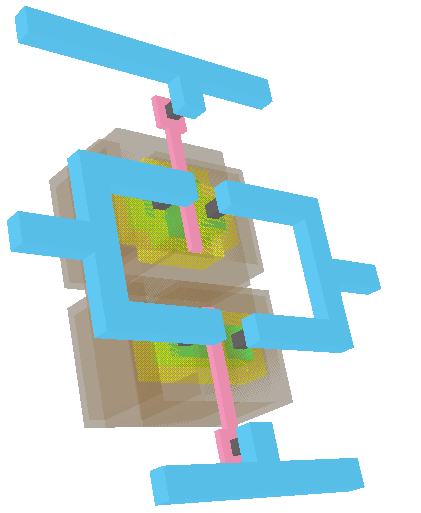
\includegraphics[scale=0.35]{pics/trans3d.png}
      \caption{Layout hecho en \textit{Electric} de una compuerta de transmisión en su vista $3D$.}
	\label{fig2}
\end{figure}
\noindent
Para la simulación se polarizó con un $V_{DD} = 5\, V$ dando como resultado
\begin{figure}[H]
  \centering
    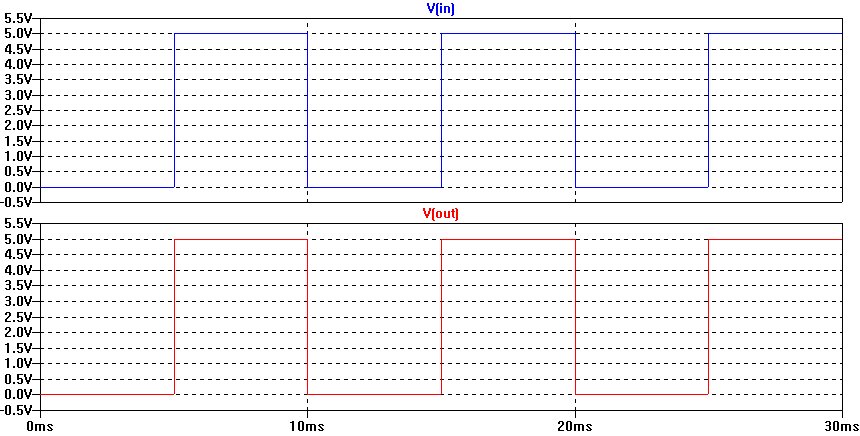
\includegraphics[scale=0.3]{pics/outtrans.png}
      \caption{Comportamiento de la compuerta transmisora del modelo SPICE.}
	\label{outinv}
\end{figure}
\begin{figure}[H]
  \centering
    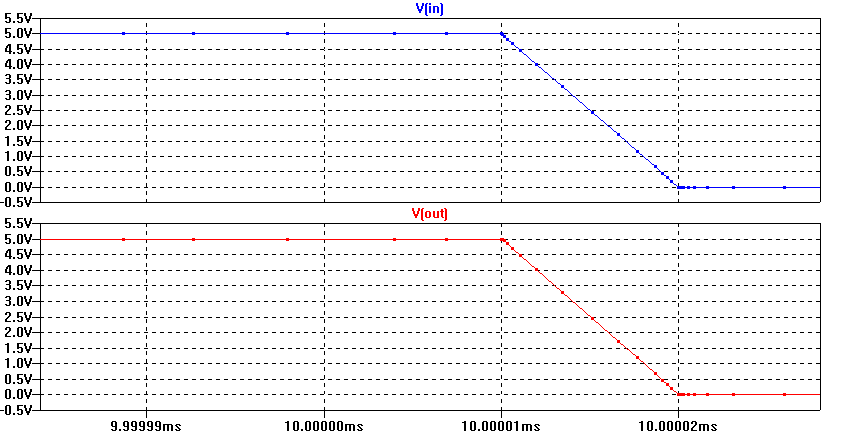
\includegraphics[scale=0.3]{pics/delay3.png}
      \caption{Retardo de las señales para $V_{DD}=5\, V$ para la compuerta de transmisión.}
	\label{delay3}
\end{figure}
\noindent

\section{Análisis de resultados y conclusiones}

\subsection{Transistores (N y P)}
\noindent
En las fig.~\ref{simP2} y \ref{simP4} es posible observar los valores de la tensión de umbral de los transistores. Se tiene por tanto \textbf{$V_{th}=-$0.9 V} y \textbf{$V_{th}=\ $0.7 V} para los transistores P y N, correspondientemente. Esto coincide por los valores del proceso C5, que son \textbf{--0.9214 V} y \textbf{0.6696 V} correspondientemente.\\\\
De igual modo, es posible a partir de las simulaciones extraer los parámetros $k_p$ y $k_n$, que no está dado explícitamente en el proceso C5. Para esto se tomaron valores de $I_d$ para diferentes valores de $V_{gs}$ en región de saturación (fig.~\ref{simP1} y \ref{simP3}). Usando entonces las ecuaciones~\ref{idn} y \ref{idp} se despeja el valor de $k_{p,n}=k^{'}W/L$. Se tiene entonces \textbf{$k_p=$ 33.28 $\mu A/V$} y \textbf{$k_n=$ 90.5 $\mu A/V$}.

\subsection{Inversor CMOS}



\subsection{Compuerta de Transmisión}


\bibliographystyle{ieeetran}
\begin{thebibliography}{99}
   
  \bibitem{jeager} Jaeger, Richard C. \& Blalock, Travis N.
  {\em "`Microelectronic Circuit Desing"'}.
  McGraw-Hill, Fourth Edition, 1999.
  
  \bibitem{sedra} Sedra, Adel S. \& Smith, Kenneth C.
  {\em "`Circuitos Microelectrónicos"'}.
  Oxford University Press, Cuarta Edición, 1999.
  
  
\end{thebibliography}
\end{document}